%(BEGIN_QUESTION)
% Copyright 2015, Tony R. Kuphaldt, released under the Creative Commons Attribution License (v 1.0)
% This means you may do almost anything with this work of mine, so long as you give me proper credit

Beregn nødvendig verdi for motstanden $R_1$ i denne kretsen for å få en utgangsspenning ($V_{out}$) på 8.1 volt:

$$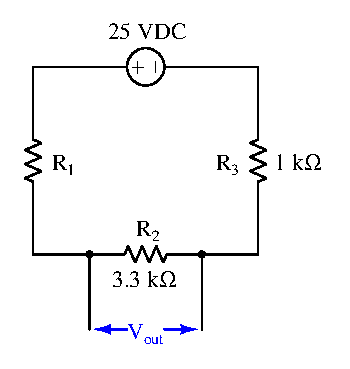
\includegraphics[width=15.5cm]{i00438x01.eps}$$

$R_1$ = 

\vskip 10pt

Marker også polariteten til $V_{out}$ med «+»- og «$-$»-symboler.

\vskip 10pt

\underbar{file i00438}
%(END_QUESTION)





%(BEGIN_ANSWER)

$R_1$ = 5.885 k$\Omega$

\vskip 10pt

$V_{out}$ er positiv til venstre og negativ til høyre.

%(END_ANSWER)





%(BEGIN_NOTES)

{\bf Dette spørsmålet er ment for eksamen og ikke for arbeidsark!}.

%(END_NOTES)
